\documentclass{article}
\usepackage[margin=0.5in]{geometry}
\usepackage{etoolbox}
\usepackage{tikz}
\usepackage{alphalph}
\usepackage{nicefrac}
\usepackage{amsmath}

\usetikzlibrary{external,shapes,calc,math,patterns,arrows,positioning,fadings}
\tikzexternalize[optimize=false]

\tikzstyle{l1}=[line width=0.9]
\tikzstyle{l2}=[line width=0.5]
\tikzstyle{node}=[circle,, draw=black, minimum size=25pt, l1, inner sep= 5pt]
\tikzstyle{nodel}=[circle, draw=black, minimum size=15pt, l1, inner sep= 0pt]
\tikzstyle{nodem}=[circle, draw=black, minimum size=12pt, l1, inner sep= 0pt]
\tikzstyle{tnode}=[nodel, minimum size=0.8 cm, fill=white]
\tikzstyle{node1}=[circle, draw=black, minimum size=20pt, l1, inner sep= 2pt]
\tikzstyle{node2}=[circle, draw=black, minimum size=14pt, l1, inner sep= 0pt, fill=white!70!black]
\tikzfading[name=fade right, left color=transparent!0, right color=transparent!100]
\tikzstyle{odd}=[node2, pattern=crosshatch dots, pattern color=mred!75!white]
\tikzstyle{even}=[node2, pattern=dots, pattern color=mblue!75!white]
\tikzstyle{odd1}=[nodel, minimum size=13pt, pattern=crosshatch dots, pattern color=mred!75!white]
\tikzstyle{even1}=[nodel, minimum size=13pt, pattern=dots, pattern color=mblue!75!white]
\tikzstyle{lodd}=[odd, pattern = crosshatch dots]
\tikzstyle{leven}=[even, pattern = crosshatch dots]
\tikzstyle{enset}=[node1, thick, double, font=\footnotesize, fill=white]
\tikzstyle{onset}=[node1, thick, densely dashed, double, font=\footnotesize, fill=white]
\tikzstyle{subtree}=[node1, opacity=0.3,dotted, font=\footnotesize]
\tikzstyle{known}=[nodel, pattern=dots, pattern color=green!75!white]
\tikzstyle{undef}=[nodel, dotted, pattern=dots, pattern color=black!25!white]
\tikzstyle{edge}=[above,midway,font=\tiny]
\tikzstyle{smallarrow} = [draw, single arrow, shape border rotate=270, minimum height=0.25cm, minimum width=0.35cm, single arrow head extend=0.01cm, inner sep=0]
\tikzstyle{legend} = [fill=mgrey, fill opacity=.1, rounded corners]
\tikzstyle{parameters} = [draw, l1, align=left, opacity=0.5, text opacity=1, font=\footnotesize]
\tikzstyle{delay} = [l2, densely dashed, color=mpink]
\tikzstyle{parity} = [l2, densely dotted, color=mblue]

\newcommand\DLINE[4]{
  \draw (#1, #2) ++ (-.3,-.9) node[inner sep=0] (lb) {} ++(#3,0) ++(.6,0) node[inner sep=0] (rb) {} ++(0,0.4) node[inner sep=0] (rt) {};;
  \path[fill=white!80!black, rounded corners=2pt] (lb) rectangle (rt);
  \ifnumequal{#4}{1}{\draw[thin] (lb) -- (rb);}{}
}

\usepackage{xcolor}
\definecolor{mblue}{HTML}{1F77B4}
\definecolor{morange}{HTML}{FF7F0E}
\definecolor{mgreen}{HTML}{2CA02C}
\definecolor{mred}{HTML}{D62728}
\definecolor{mpurple}{HTML}{9467BD}
\definecolor{mbrown}{HTML}{8C564B}
\definecolor{mpink}{HTML}{E377C2}
\definecolor{mgrey}{HTML}{7F7F7F}
\definecolor{mlime}{HTML}{BCBD22}
\definecolor{mcyan}{HTML}{17BECF}

% Set new commands
\let\oldemptyset\emptyset
\let\emptyset\varnothing
\newcommand{\codefunc}[1]{\texttt{#1}}
\newcommand{\m}[1]{\mathcal{#1}}
\newcommand{\n}[1]{\mathscr{#1}}
\newcommand{\bound}{\mathscr{B}}
\newcommand{\akker}{\mathscr{A}}
\newcommand{\nset}{\mathcal{N}}
\newcommand{\vset}{\mathcal{V}}
\newcommand{\pr}[1]{ {}^{#1} }
\newcommand{\ceil}[1]{{\left \lceil #1 \right \rceil }}
\newcommand{\floor}[1]{{\left \lfloor #1 \right \rfloor }}
\DeclareMathOperator{\Find}{Find}
\DeclareMathOperator{\Union}{Union}
\DeclareMathOperator{\Nodejoin}{Join}
\DeclareMathOperator{\Support}{Support}

\begin{document}

% PMW
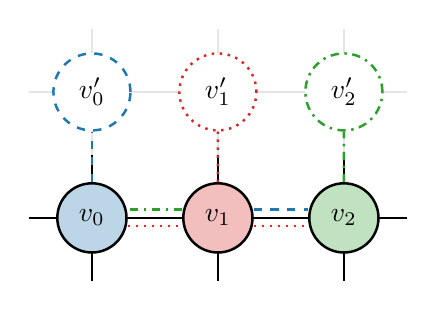
\begin{tikzpicture}[scale=0.8]
    % \node at (-1, -1) {$\mathcal{V}$};
    \draw[l1, opacity=0.1, step=2] (-1,-1) grid (5,3); 
    \draw[l1] (0, 0) -- (4,0);
    \draw[l1] (-1,0) -- (5,0);
    \draw[l1] (0,1) -- (0,-1);
    \draw[l1] (2,1) -- (2,-1);
    \draw[l1] (4,1) -- (4,-1);
    \node[node, fill=white!70!mblue, text opacity=1] at (0,0) (1) {$v_0$};
    \node[node, fill=white, draw=mblue, dashed] at (0,2) (2) {$v_0'$};
    \node[node, fill=white!70!mred, text opacity=1] at (2,0) (3){$v_1$};
    \node[node, fill=white, draw=mred,dotted] at (2,2) (4) {$v_1'$};
    \node[node, fill=white!70!mgreen, text opacity=1] at (4,0) (5) {$v_2$};
    \node[node, fill=white, draw=mgreen, dashdotted] at (4,2) (6) {$v_2'$};

    \draw[l1, dashed, mblue] (1) -- (2);
    \draw[l1, dashed, mblue, transform canvas={yshift=3pt}] (3) -- (5);
    \draw[l1, dotted, mred] (3) -- (4);
    \draw[l1, dotted, mred, transform canvas={yshift=-3pt}] (1) -- (3) -- (5);
    \draw[l1, dashdotted, mgreen] (5) -- (6);
    \draw[l1, dashdotted, mgreen, transform canvas={yshift=3pt}] (3) -- (1);
\end{tikzpicture}


% Node-tree
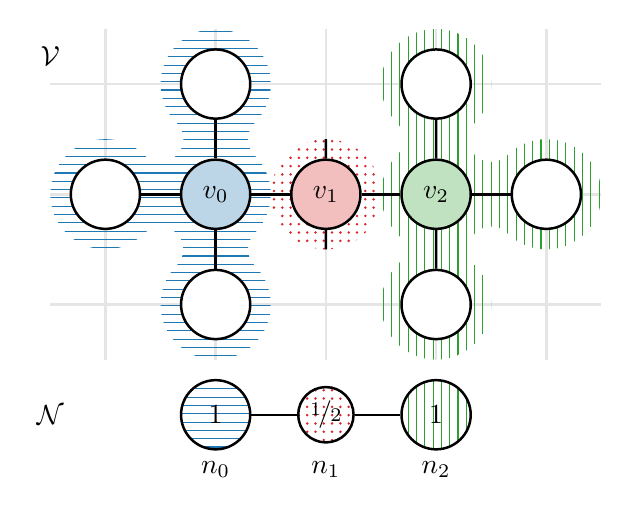
\begin{tikzpicture}[scale=0.7]
    \draw[l1, opacity=0.1, step=2] (-3,-3) grid (7,3); 

    \path[pattern=horizontal lines, pattern color=mblue] (0,3) arc (90:225:1) arc (45:-135:.4142) arc (45:315:1) arc (135:-45:.4142) arc (135:405:1) arc (225:135:.4142) arc (-45:45:1) arc (225:135:.4142) arc (-45:90:1) -- cycle;

    \begin{scope}[shift={(4,0)}, xscale=-1]
        \path[pattern=vertical lines, pattern color=mgreen] (0,3) arc (90:225:1) arc (45:-135:.4142) arc (45:315:1) arc (135:-45:.4142) arc (135:405:1) arc (225:135:.4142) arc (-45:45:1) arc (225:135:.4142) arc (-45:90:1) -- cycle;
    \end{scope}
    \path[pattern=dots , pattern color=mred] (2,1) arc (90:450:1);

    \node[node, fill=white!70!mblue] at (0,0) (0) {$v_0$};
    \node[node, fill=white!70!mred] at (2,0) (1) {$v_1$};
    \node[node, fill=white!70!mgreen] at (4,0) (5) {$v_2$};
    \node[node, fill=white] at (-2,0) (2) {};
    \node[node, fill=white] at (0,2) (3) {};
    \node[node, fill=white] at (0,-2) (4) {};
    \node[node, fill=white] at (6,0) (6) {};
    \node[node, fill=white] at (4,2) (7) {};
    \node[node, fill=white] at (4,-2) (8) {};

    % \draw[l1] (2) -- +(-1,0) (2) -- +(0,1) (2) -- +(0,-1);
    % \draw[l1] (3) -- +(1,0) (3) -- +(-1,0) (3) -- +(0,1);
    % \draw[l1] (4) -- +(1,0) (4) -- +(-1,0) (4) -- +(0,-1);
    % \draw[l1] (6) -- +(1,0) (6) -- +(0,1) (6) -- +(0,-1);
    % \draw[l1] (7) -- +(1,0) (7) -- +(-1,0) (7) -- +(0,1);
    % \draw[l1] (8) -- +(1,0) (8) -- +(-1,0) (8) -- +(0,-1);

    \draw[l1] (6) -- (5) -- (1) -- (0) -- (3);
    \draw[l1] (2) -- (0) -- (4);
    \draw[l1] (7) -- (5) -- (8);
    \draw[l1] (2, 1) -- (1) -- (2,-1);
    \node at (-3, 2.5) {$\mathcal{V}$};

    \begin{scope}[shift={(0, -4)}]
        \node at (-3, 0) {$\mathcal{N}$};
        \node[node, pattern=horizontal lines, pattern color=mblue] at (0,0) (d) {$1$};
        \node[node1, inner sep=0, pattern=dots , pattern color=mred] at (2,0) (e) {$\nicefrac{1}{2}$};
        \node[node, pattern=vertical lines, pattern color=mgreen] at (4,0) (f) {$1$};
        \node at (0,-1) {$n_0$};
        \node at (2,-1) {$n_1$};
        \node at (4,-1) {$n_2$};
        \draw[l1] (d) -- (e) -- (f);
    \end{scope}
\end{tikzpicture}


% Node types
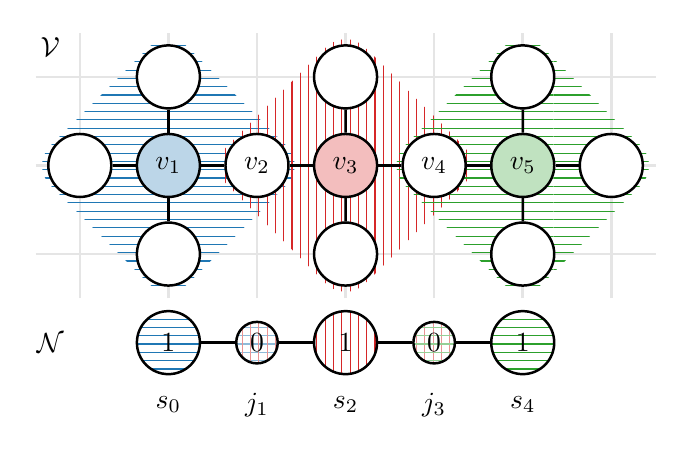
\begin{tikzpicture}[scale=0.75]
    
    \node at (-3, 2) {$\mathcal{V}$};
    \node at (-3, -3) {$\mathcal{N}$};
    \begin{scope}[shift={(-1, 0)}, scale=1.5]
        \draw[l1, opacity=0.1, step=1] (-1.5,-1.5) grid (5.5,1.5); 
        \node at (0,0) (0) {}; \node at (2,0) (1) {}; \node at (4,0) (2) {};
        \path[pattern=horizontal lines, pattern color=mblue, rounded corners=10pt, rotate around={45:(0)}] (-1.1,-1.1) rectangle (1.1,1.1);
        \path[pattern=vertical lines, pattern color=mred, rounded corners=10pt, rotate around={45:(1)}] (0.9,-1.1) rectangle (3.1,1.1);
        \path[pattern=horizontal lines, pattern color=mgreen, rounded corners=10pt, rotate around={45:(2)}] (2.9,-1.1) rectangle (5.1,1.1);

        \node[tnode, fill=white!70!mblue] at (0) (v0) {$v_1$};
        \node[tnode] at (-1,0) (v0l) {};
        \node[tnode] at (0,1) (v0u) {};
        \node[tnode] at (0,-1) (v0d) {};

        \node[tnode, fill=white!70!mred] at (1) (v1) {$v_3$};
        \node[tnode] at (1,0) (v1l) {$v_{2}$};
        \node[tnode] at (2,1) (v1u) {};
        \node[tnode] at (2,-1) (v1d) {};

        \node[tnode, fill=white!70!mgreen] at (2) (v2) {$v_5$};
        \node[tnode] at (3,0) (v2l) {$v_{4}$};
        \node[tnode] at (5,0) (v2r) {};
        \node[tnode] at (4,1) (v2u) {};
        \node[tnode] at (4,-1) (v2d) {};

        \draw[l1] (v0l) -- (v0) -- (v1l) -- (v1) -- (v2l) -- (v2) -- (v2r);
        \draw[l1] (v0u) -- (v0) -- (v0d);
        \draw[l1] (v1u) -- (v1) -- (v1d);
        \draw[l1] (v2u) -- (v2) -- (v2d);
    \end{scope}

    \begin{scope}[shift={(-1, -3)}, scale=1.5]
        \node[tnode, pattern=horizontal lines, pattern color=mblue] at (0,0) (n0) {1};
        \node[nodel, pattern=horizontal lines, pattern color=mblue!50!white, line width=0] at (1,0) {};
        \node[nodel, pattern=vertical lines,   pattern color=mred!50!white] at (1,0) (j01) {0};
        \node[tnode, pattern=vertical lines , pattern color=mred] at (2,0) (n1) {1};
        \node[nodel, pattern=vertical lines,   pattern color=mred!50!white, line width=0] at (3,0) {};
        \node[nodel, pattern=horizontal lines, pattern color=mgreen!50!white] at (3,0) (j12) {0};
        \node[tnode, pattern=horizontal lines, pattern color=mgreen] at (4,0) (n2) {1};
        \node at (0,-.7) {$s_0$};
        \node at (1,-.7) {$j_{1}$};
        \node at (2,-.7) {$s_2$};
        \node at (3,-.7) {$j_{3}$};
        \node at (4,-.7) {$s_4$};
        \draw[l1] (n0) -- (j01) -- (n1) -- (j12) -- (n2);
    \end{scope}
\end{tikzpicture}

% DFS
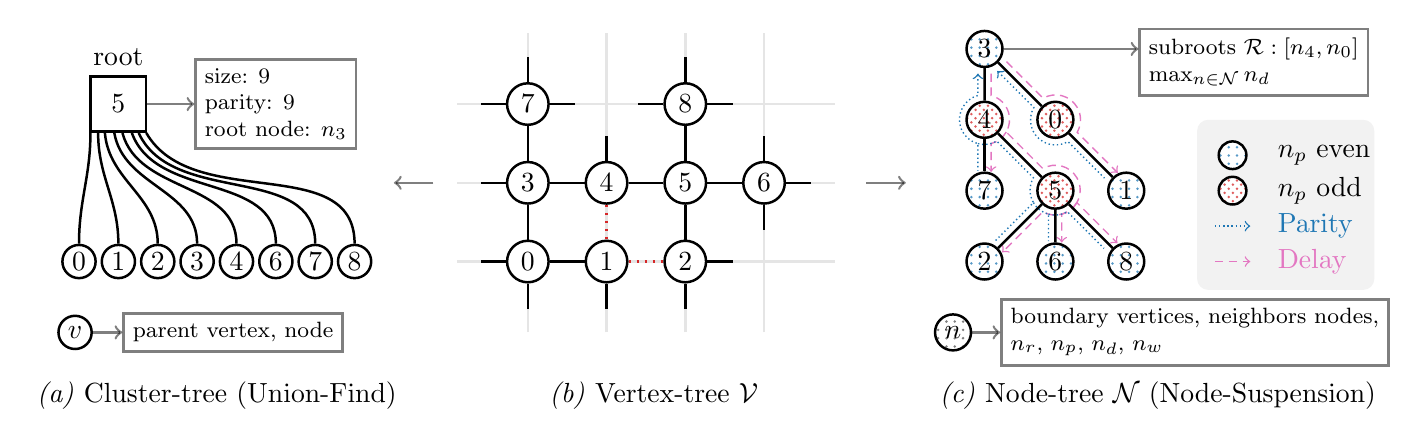
\begin{tikzpicture}[x=1cm,y=1cm]

    % \node at (-2.75, -1.7) {\emph{(a)} Cluster-tree (Union-Find)};
    % \node at (3.1, -1.7) {\emph{(b)} Vertex-tree $\vset$};
    % \node at (9.2,-1.7) {\emph{(c)} Node-tree $\mathcal{N}$ (Node-Suspension)};
    % \begin{scope}[scale=0.8, shift={(2.2,.7)}]
    %     \draw[l1, opacity=0.1, step=1] (-.9,-.9) grid (3.9,2.9);
    %     \node [nodel, fill=white] (w0) at (0,0) {$0$};
    %     \node [nodel, fill=white] (w1) at (1,0) {$1$};
    %     \node [nodel, fill=white] (w2) at (2,0) {$2$};
    %     \node [nodel, fill=white] (w3) at (0,1) {$3$};
    %     \node [nodel, fill=white] (w4) at (1,1) {$4$};
    %     \node [nodel, fill=white] (w5) at (2,1) {$5$};
    %     \node [nodel, fill=white] (w7) at (0,2) {$7$};
    %     \node [nodel, fill=white] (w8) at (2,2) {$8$};
    %     \node [nodel, fill=white] (w6) at (3,1) {$6$};
    %     \draw [l1] (w7) -- (w3) -- (w0) -- (w1) (w3) -- (w4) -- (w5) -- (w8) (w6) -- (w5) -- (w2);
    %     \draw [l1] (w0) -- +(-.6,0) (w0) -- +(0, -.6);
    %     \draw [l1] (w3) -- +(-.6,0);
    %     \draw [l1] (w7) -- +(-.6,0) (w7) -- +(0, .6) (w7) -- +(0.6, 0);
    %     \draw [l1] (w4) -- +(0, .6);
    %     \draw [l1] (w8) -- +(-.6,0) (w8) -- +(0, .6) (w8) -- +(0.6, 0);
    %     \draw [l1] (w6) -- +(0,-.6) (w6) -- +(0, .6) (w6) -- +(0.6, 0);
    %     \draw [l1] (w2) -- +(.6,0) (w2) -- +(0, -.6);
    %     \draw [l1] (w1) -- +(0,-.6);
    %     \draw [l1, dotted, mred] (w4) -- (w1) -- (w2);
    % \end{scope}
    % \draw[l1, opacity=0.5, ->] (5.5,1) -- +(.5,0);
    % \draw[l1, opacity=0.5, ->] (0.5,1) -- +(-.5,0);

    \draw[l1, opacity=0.5, ->] (5.5,1) -- +(.5,0);
    \draw[l1, opacity=0.5, ->] (0,1) -- +(-.5,0);
    \begin{scope}[shift={(-2.75, -1.7)}]
        \node at (0,0) {\emph{(a)} Cluster-tree (Union-Find)};
        \node[nodem, minimum size=12] (v) at (-1.8,.8){$v$};
        \node[parameters, anchor=west] (vi) at (-1.2,.8){parent vertex, node}; 
        \draw[l1, opacity=0.5, ->] (v) -- (vi);
    \end{scope}
    \begin{scope}[shift={(2.8, -1.7)}]
        \node at (0,0) {\emph{(b)} Vertex-tree $\vset$};
    \end{scope}
    \begin{scope}[shift={(9.2,-1.7)}]
        \node at (0,0) {\emph{(c)} Node-tree $\mathcal{N}$ (Node-Suspension)};
        \node[even1, pattern color=mgrey] (n) at (-2.6,.8){$n$};
        \node[parameters, anchor=west, align=left] (ni) at (-2,.8){boundary vertices, neighbors nodes,\\ $n_r$, $n_p$, $n_d$, $n_w$}; 
        \draw[l1, opacity=0.5, ->] (n) -- (ni);
    \end{scope}

    \begin{scope}[scale=1, shift={(1.2,0)}]
        \draw[l1, opacity=0.1, step=1] (-.9,-.9) grid (3.9,2.9);
        \node [nodel, fill=white] (w0) at (0,0) {$0$};
        \node [nodel, fill=white] (w1) at (1,0) {$1$};
        \node [nodel, fill=white] (w2) at (2,0) {$2$};
        \node [nodel, fill=white] (w3) at (0,1) {$3$};
        \node [nodel, fill=white] (w4) at (1,1) {$4$};
        \node [nodel, fill=white] (w5) at (2,1) {$5$};
        \node [nodel, fill=white] (w7) at (0,2) {$7$};
        \node [nodel, fill=white] (w8) at (2,2) {$8$};
        \node [nodel, fill=white] (w6) at (3,1) {$6$};
        \draw [l1] (w7) -- (w3) -- (w0) -- (w1) (w3) -- (w4) -- (w5) -- (w8) (w6) -- (w5) -- (w2);
        \draw [l1] (w0) -- +(-.6,0) (w0) -- +(0, -.6);
        \draw [l1] (w3) -- +(-.6,0);
        \draw [l1] (w7) -- +(-.6,0) (w7) -- +(0, .6) (w7) -- +(0.6, 0);
        \draw [l1] (w4) -- +(0, .6);
        \draw [l1] (w8) -- +(-.6,0) (w8) -- +(0, .6) (w8) -- +(0.6, 0);
        \draw [l1] (w6) -- +(0,-.6) (w6) -- +(0, .6) (w6) -- +(0.6, 0);
        \draw [l1] (w2) -- +(.6,0) (w2) -- +(0, -.6);
        \draw [l1] (w1) -- +(0,-.6);
        \draw [l1, dotted, mred] (w4) -- (w1) -- (w2);
    \end{scope}


    

    \begin{scope}[shift={(-3,0)}]
        \node at (-1, 2.6) {root};
        \node[draw, l1, minimum size=20]   (v0) at (-1,2){$5$};
        \node[nodem, minimum size=12] (v1) at (-1.5,0){$0$};
        \node[nodem, minimum size=12] (v2) at (-1,0)  {$1$};
        \node[nodem, minimum size=12] (v3) at (-.5,0) {$2$};
        \node[nodem, minimum size=12] (v4) at (0,0)   {$3$};
        \node[nodem, minimum size=12] (v5) at (.5,0)  {$4$};
        \node[nodem, minimum size=12] (v6) at (1,0)   {$6$};
        \node[nodem, minimum size=12] (v7) at (1.5,0) {$7$};
        \node[nodem, minimum size=12] (v8) at (2,0)   {$8$};
        \draw[l1] (v1) to [out=90, in=270] (v0.226);
        \draw[l1] (v2) to [out=90, in=270] (v0.235);
        \draw[l1] (v3) to [out=90, in=275] (v0.245);
        \draw[l1] (v4) to [out=90, in=280] (v0.262);
        \draw[l1] (v5) to [out=90, in=285] (v0.278);
        \draw[l1] (v6) to [out=90, in=290] (v0.295);
        \draw[l1] (v7) to [out=90, in=295] (v0.305);
        \draw[l1] (v8) to [out=90, in=300] (v0.314);

        \node[parameters] (inf) at (1,2) {size: 9\\parity: 9\\root node: $n_3$};
        \draw[l1, ->, opacity=.5] (v0) -- (inf);
    \end{scope}

    \begin{scope}[shift={(7,0)}, scale=0.9]
        % \node at (0.3, 3) {$\nset_r$};
        \node[even1] (a) at (0, 3) {3};
        \node[odd1]  (b) at (0, 2) {4};
        \node[odd1]  (c) at (1, 1) {5};
        \node[even1] (d) at (1, 0) {6};
        \node[even1] (e) at (0, 1) {7};
        \node[even1] (f) at (0, 0) {2};
        \node[odd1]  (g) at (1, 2) {0};
        \node[even1] (h) at (2, 1) {1};
        \node[even1] (i) at (2, 0) {8};

        \draw[delay, ->] (a.-30) ++(-30:2.5pt) -- ++(-45:0.73cm) arc (120:-30:10pt) -- ++(-45:0.81cm);
    
        \draw[delay, ->] (a.-75) ++(-75:2.5pt) -- ++(0,-.31cm) arc (75:-30:10pt) node (d4){} -- ++(-45:0.73cm) arc (120:-30:10pt) node (d5){} -- ++(-45:0.81cm);
        \draw[delay, ->] (d4) arc (-30:-75:10pt) -- ++(0,-.4cm);
        \draw[delay, ->] (d5) arc (-30:-75:10pt) -- ++(0,-.4cm);
        \draw[delay, ->] (d5) arc (-30:-120:10pt) -- ++(-135:0.81cm);
        \draw[parity, <-] (a.-60) ++(-60:2.5pt) -- ++(-45:0.73cm) arc (150:300:10pt) -- ++(-45:0.73cm);
        \draw[parity, <-] (a.-105) ++(-105:2.5pt) -- ++(0,-.31cm) arc(105:255:10pt) node (p4){} -- ++(0,-.38cm);
        \draw[parity] (p4) arc (-105:-60:10pt) -- ++(-45:0.73cm) arc (150:210:10pt) node (p5){} -- ++(-135:0.76cm);
        \draw[parity] (p5) arc (210:255:10pt) node (p5b) {} -- ++(0,-.38cm);
        \draw[parity] (p5b) arc(255:300:10pt) -- ++(-45:0.73cm);
        
        % -- ++(-45:0.73cm) arc (150:300:10pt) -- ++(-45:0.73cm);
        
        \draw[l1] (a) -- (b) -- (c) -- (d);
        \draw[l1] (b) -- (e);
        \draw[l1] (c) -- (f);
        \draw[l1] (c) -- (i);
        \draw[l1] (a) -- (g) -- (h);


        % \node[text=morange] at (2.6,2.8) {Delay};
        \node[parameters, anchor=north] (inf2) at (3.8,3.3) {subroots $\m{R}: [n_4, n_0]$\\$\max_{n \in \nset}{n_d}$};
        \draw[l1, ->, opacity=.5] (a) -- (a-|inf2.west);
        
        
        \begin{scope}[shift={(3.5,0)}]
            \path[legend] (-.5, 2) rectangle (2, -.4);
            \path (0,1.5) node[even1, minimum size=10, preaction={fill, white}]{} -- +(.5,0) node[anchor=west] {$n_p$ even};
            \path (0,1) node[odd1 , minimum size=10, preaction={fill, white}]{} -- +(.5,0) node[anchor=west] {$n_p$ odd};
            \draw[parity, ->] (-.25, .5) -- ++(0.5,0);
            \draw[delay, ->] (-.25, 0) -- ++(0.5,0);
            \node[color=mblue, anchor=west] at (.5,.5) {Parity};
            \node[color=mpink, anchor=west] at (.5,0) {Delay};
        \end{scope}
    \end{scope}

    
\end{tikzpicture}



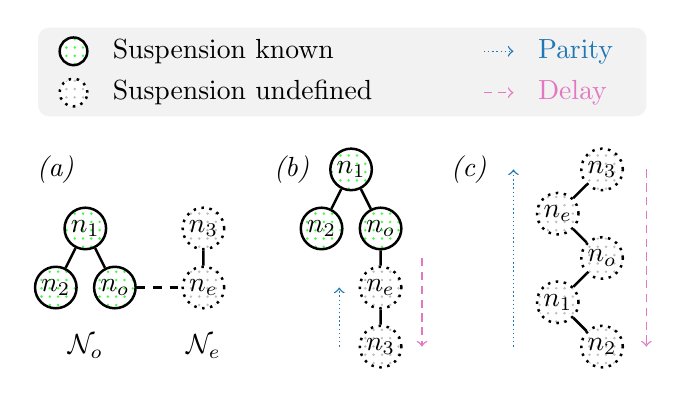
\begin{tikzpicture}[scale=0.75]
    \begin{scope}[shift={(0,-1)}]
        \node at (1.5,-1) {$\nset_o$};
        \node at (3.5,-1) {$\nset_e$};
        \node (o1) [known] at (1.5, 1) {$n_1$};
        \node (o2) [known] at (1, 0) {$n_2$};
        \node (o3) [known] at (2, 0) {$n_o$};
        \node (e4) [undef] at (3.5,1) {$n_3$};
        \node (e5) [undef] at (3.5,0) {$n_e$};
        \draw[l1] (o2) -- (o1) -- (o3) (e4) -- (e5);
        \draw[l1, dashed] (o3) -- (e5) node[midway,below] (a) {};
        % \draw[l1, <-] (a) -- ++(0,-.5) node[below] {$\Nodejoin(n_e, n_o)$};
    \end{scope}

    \begin{scope}[shift={(4.5,0)}]
        \node (o1) [known] at (1.5, 1) {$n_1$};
        \node (o2) [known] at (1, 0) {$n_2$};
        \node (o3) [known] at (2, 0) {$n_o$};
        \node (e4) [undef] at (2,-2) {$n_3$};
        \node (e5) [undef] at (2,-1) {$n_e$};
        \draw[l1] (o2) -- (o1) -- (o3) -- (e5) -- (e4);
        \draw[parity, ->] (e4) ++(-.7,0) -- + (0,1);
        \draw[delay, ->] (o3) ++(.7,-.5) -- +(0,-1.5);
    \end{scope}

    \begin{scope}[shift={(9.5,-2)}]
        \node (o1) [undef] at (0, 0.75) {$n_1$};
        \node (o2) [undef] at (0.75, 0) {$n_2$};
        \node (o3) [undef] at (0.75, 1.5) {$n_o$};
        \node (e4) [undef] at (0.75,3) {$n_3$};
        \node (e5) [undef] at (0,2.25) {$n_e$};
        \draw[l1] (o2) -- (o1) -- (o3) -- (e5) -- (e4);
        \draw[parity, <-] (e4) ++(-1.5,0) -- +(0,-3);
        \draw[delay, ->] (e4) ++(.75,0) -- +(0,-3);
    \end{scope}

    \node at (1,1) {\emph{(a)}};
    \node at (5,1) {\emph{(b)}};
    \node at (8,1) {\emph{(c)}};
    % \draw[l1, opacity=0.5, ->, text opacity=1] (8.5,-2) -- +(0,-.5) node[midway, right] {$n_3$};
    % \draw[l1, opacity=0.5, ->, text opacity=1] (6.5,-2) -- +(-.3,-.5) node[midway, left=.1] {New root node = \hspace{0.5cm} $n_1$};

    \begin{scope}[shift={(1,1)}]

        \path[legend] (-.3,0.9) rectangle (10,2.4);
        \path (.3, 2) node[known, minimum size=10, preaction={fill, white}] {} -- +(.5,0) node[anchor=west, align=left]{Suspension known};
        \path (.3, 1.3) node[undef, minimum size=10, preaction={fill, white}] {} -- +(.5,0) node[anchor=west, align=left]{Suspension undefined};
        \draw[parity, ->] (7.25,2) -- ++(0.5,0);
        \node[color=mblue, anchor=west] at (8,2) {Parity};
        \draw[delay, ->] (7.25, 1.3) -- ++(0.5,0);
        \node[color=mpink, anchor=west] at (8,1.3) {Delay};
        
    \end{scope}

\end{tikzpicture}

% Equilibrium

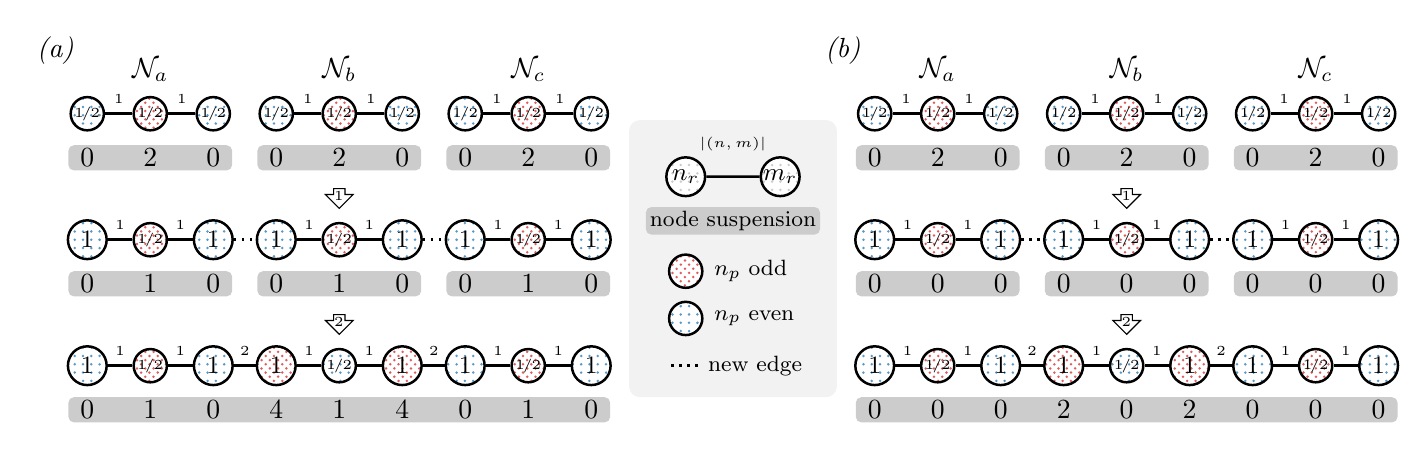
\begin{tikzpicture}[on grid, scale=0.8]

    \begin{scope}[shift={(9.5,-3)}]
        \path[legend] (-.9, -1.5) rectangle (2.4, 2.9);
        \node[node2, pattern=dots, pattern color=black!20!white, preaction={fill, white}] (n1) at (0,2) {\small$n_r$};
        \node[node2, pattern=dots, pattern color=black!20!white, preaction={fill, white}] (n2) at (1.5,2) {\small$m_r$};
        \draw[l1] (n1) -- (n2) node[edge, above=0.2cm]{$|(n, m)|$};
        \node[align=center, fill=white!80!black, rounded corners=2pt, inner sep=0.5mm] at (0.75, 1.3) {\footnotesize node suspension};
        \draw (0, 0.5) node[odd, nodem, preaction={fill, white}]{} +(.3,0) node[align=left, anchor=west]{\footnotesize $n_p$ odd };
        \draw (0, -0.25) node[even, nodem, preaction={fill, white}]{} +(.3,0) node[align=left, anchor=west]{\footnotesize $n_p$ even };
        \node[minimum size=10pt] (l) at (0, -1) {};
        \node[align=left, anchor=west] at (.2,-1) {\footnotesize new edge};
        \draw[l1, dotted] (l.west) -- (l.east);
    \end{scope}

    \node at (-.5,1) {\emph{(a)}};
    \node[smallarrow, label={[label distance=-3.6mm]0:\tiny 1}] at (4, -1.3) {};

    \foreach \x in {0,3,6}{\DLINE{\x}{0}{2}{0}}
    \foreach \x in {0,2,3,5,6,8}{\draw (\x,0) node [even, nodem] (a\x) {\tiny$\nicefrac{1}{2}$} ++(0,-.7) node (ad\x) {0};}
    \foreach[count=\i] \x in {1,4,7}{      \draw (\x,0) node [odd, nodem]  (a\x) {\tiny$\nicefrac{1}{2}$} ++(0,-.7) node (ad\x) {2};
            \node at (\x,0.7) {$\nset_{\alphalph{\i}}$};}
    \draw[l1] (a0) -- (a1) node[edge]{1} -- (a2) node[edge]{1} (a3) -- (a4) node[edge]{1} -- (a5) node[edge]{1} (a6) -- (a7) node[edge]{1} -- (a8) node[edge]{1};

    \begin{scope}[shift={(0,-2)}]
        \node[smallarrow, label={[label distance=-3.6mm]0:\tiny 2}] at (4, -1.3) {};
        \foreach \x in {0,3,6}{\DLINE{\x}{0}{2}{0}}
        \foreach \x in {0,2,3,5,6,8}{\draw (\x,0) node [even] (e\x) {\small1} ++(0,-.7) node {0};}
        \foreach \x in {1,4,7}{      \draw (\x,0) node [odd, nodem]  (e\x) {\tiny$\nicefrac{1}{2}$} ++(0,-.7) node {1};}
        \draw[l1] (e0) -- (e1) node[edge]{1} -- (e2) node[edge]{1} (e3) -- (e4) node[edge]{1} -- (e5) node[edge]{1} (e6) -- (e7) node[edge]{1} -- (e8) node[edge]{1};
        \draw[l1, dotted] (e2) -- (e3) (e5) -- (e6);
    \end{scope}

    \begin{scope}[shift={(0,-4)}]
        \DLINE{0}{0}{8}{0}
        \foreach \x in {0,2,6,8}{\draw (\x,0) node [even] (b\x) {\small1} ++(0,-.7) node {0};}
        \foreach \x in {1,7}{    \draw (\x,0) node [odd, nodem]  (b\x) {\tiny$\nicefrac{1}{2}$} ++(0,-.7) node {1};}
        \foreach \x in {3,5}{    \draw (\x,0) node [odd]  (b\x) {\small1} ++(0,-.7) node {4};}
        \draw (4,0)  node [even, nodem] (b4)  {\tiny$\nicefrac{1}{2}$} ++(0,-.7) node {1};
        \draw[l1] (b0) -- (b1) node[edge]{1} -- (b2) node[edge]{1} -- (b3) node[edge]{2} -- (b4) node[edge]{1} -- (b5) node[edge]{1} -- (b6) node[edge]{2} -- (b7) node[edge]{1} -- (b8) node[edge]{1};
    \end{scope}


    \begin{scope}[shift={(12.5,0)}]
        \node at (-.5,1) {\emph{(b)}};
        \node[smallarrow, label={[label distance=-3.6mm]0:\tiny 1}] at (4, -1.3) {};

        \foreach \x in {0,3,6}{\DLINE{\x}{0}{2}{0}}
        \foreach \x in {0,2,3,5,6,8}{\draw (\x,0) node [even, nodem] (c\x) {\tiny$\nicefrac{1}{2}$} ++(0,-.7) node {0};}
        \foreach[count=\i] \x in {1,4,7}{      \draw (\x,0) node [odd, nodem]  (c\x) {\tiny$\nicefrac{1}{2}$} ++(0,-.7) node (cd\x) {2};
                \node at (\x,0.7) {$\nset_{\alphalph{\i}}$};}
        \draw[l1] (c0) -- (c1) node[edge]{1} -- (c2) node[edge]{1} (c3) -- (c4) node[edge]{1} -- (c5) node[edge]{1} (c6) -- (c7) node[edge]{1} -- (c8) node[edge]{1};

        \begin{scope}[shift={(0,-2)}]
            \node[smallarrow, label={[label distance=-3.6mm]0:\tiny 2}] at (4, -1.3) {};
            \foreach \x in {0,3,6}{\DLINE{\x}{0}{2}{0}}
            \foreach \x in {0,2,3,5,6,8}{\draw (\x,0) node [even] (c\x) {\small1} ++(0,-.7) node {0};}
            \foreach \x in {1,4,7}{      \draw (\x,0) node [odd, nodem]  (c\x) {\tiny$\nicefrac{1}{2}$} ++(0,-.7) node {0};}
            \draw[l1] (c0) -- (c1) node[edge]{1} -- (c2) node[edge]{1} (c3) -- (c4) node[edge]{1} -- (c5) node[edge]{1} (c6) -- (c7) node[edge]{1} -- (c8) node[edge]{1};
            \draw[l1, dotted] (c2) -- (c3) (c5) -- (c6);
        \end{scope}

        \begin{scope}[shift={(0,-4)}]
            \DLINE{0}{0}{8}{0}
            \foreach \x in {0,2,6,8}{\draw (\x,0) node [even] (d\x) {\small1} ++(0,-.7) node {0};}
            \foreach \x in {1,7}{    \draw (\x,0) node [odd, nodem]  (d\x) {\tiny$\nicefrac{1}{2}$} ++(0,-.7) node {0};}
            \foreach \x in {3,5}{    \draw (\x,0) node [odd]  (d\x) {\small1} ++(0,-.7) node {2};}
            \draw (4,0)  node [even, nodem] (d4)  {\tiny$\nicefrac{1}{2}$} ++(0,-.7) node {0};
            \draw[l1] (d0) -- (d1) node[edge]{1} -- (d2) node[edge]{1} -- (d3) node[edge]{2} -- (d4) node[edge]{1} -- (d5) node[edge]{1} -- (d6) node[edge]{2} -- (d7) node[edge]{1} -- (d8) node[edge]{1};
        \end{scope}
    \end{scope}
\end{tikzpicture}

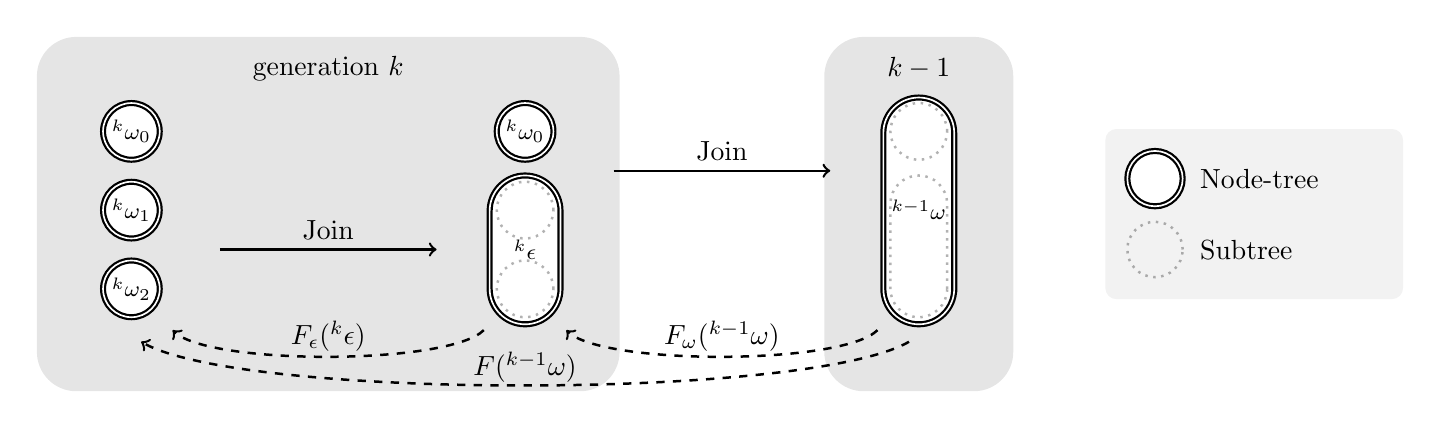
\begin{tikzpicture}[scale=.9, node distance=1cm, on grid]

    \node (a) at (0,0) {};
    \node (b) [right = 5cm of a] {};
    \node (c) [right = 5cm of b] {};
    \node (d) [right = 3cm of c] {};

    \node (b1l) [below left = 1.3cm and 1.2cm of a] {};
    \node (b1r) [above right = 3.2cm and 1.2cm of b] {};
    \path[fill=black!10!white, rounded corners=0.5cm] (b1l) rectangle (b1r);
    \node (b1t) at ($(a)!0.5!(b)$) {}; \node [above=2.8cm of b1t] {generation $k$};
    \node (b2l) [below left = 1.3cm and 1.2cm of c] {};
    \node (b2r) [above right = 3.2cm and 1.2cm of c] {};
    \path[fill=black!10!white, rounded corners=0.5cm] (b2l) rectangle (b2r);
    \node [above=2.8cm of c] {$k-1$};

    \node (l) [above=.5cm of d] {};
    \begin{scope}[shift={(l)}]
        \path[legend] (-.7,-.7) rectangle (3.5,1.7);
        % \path (0,2) node[enset]{} -- +(.5,0)node[anchor=west]{odd node-tree};
        \path (0,1) node[enset]{} -- +(.5,0)node[anchor=west]{Node-tree};
        \path (0,0) node[subtree]{} -- +(.5,0)node[anchor=west]{Subtree};
    \end{scope}

    \node (a0) [above = 0 cm of a] {};
    \node (a1) [above = 1 cm of a] {};
    \node (a2) [above = 2 cm of a] {};
    \draw[enset] (a0) circle[radius=.4cm];
    \draw[enset] (a1) circle[radius=.4cm];
    \draw[enset] (a2) circle[radius=.4cm];
    \node at (a0) {\footnotesize $\pr{k}\omega_2$};
    \node at (a1) {\footnotesize $\pr{k}\omega_1$};
    \node at (a2) {\footnotesize $\pr{k}\omega_0$};

    \foreach \i in {0,1,2}{
            \node (b\i) [above = \i cm of b] {};
        }
    \draw[enset] (b2) circle[radius=0.4cm];
    \node at (b2) {\footnotesize $\pr{k}\omega_0$};

    \draw[enset] (b0) ++(0.5cm,0) -- ++(0, 1.1cm) arc (0:180:0.5cm) -- ++(0, -1.1cm) arc (180:360:0.5cm) -- cycle;
    \draw[subtree] (b1) circle[radius=.4cm];
    \draw[subtree] (b0) circle[radius=.4cm];
    \node at ($(b0)!0.5!(b1)$) {\footnotesize $\pr{k}\epsilon$};

    \foreach \i in {0,1,2}{
            \node (c\i) [above =\i cm of c] {};
        }

    \draw[enset] (c0) ++(0.5cm,0) -- +(0, 2.2cm) arc (0:180:0.5cm) -- +(0, -2.2cm) arc (180:360:0.5cm) -- cycle;
    \node at (c1) {\footnotesize $\pr{k-1}\omega$};

    \draw[subtree] (c2) circle[radius=.4cm];
    \draw[subtree] (c0) ++(0.4cm,0) -- +(0, 1.2) arc (0:180:0.4) -- +(0, -1.2) arc (180:360:0.4) -- cycle;


    \node (f1a) [below left = 0.4cm and 0.4cm of c] {}; \node (f1b) [below right = 0.4cm and 0.4cm of b] {};
    \node (f2a) [below left = 0.4cm and 0.4cm of b] {}; \node (f2b) [below right = 0.4cm and 0.4cm of a] {};
    \node (fa) [below = 0.6cm of c] {}; \node (fb) [below = 0.6cm of a] {};
    \draw[l1, ->, dashed] (f1a) .. controls +(225:0.9cm) and +(315:0.9cm) .. (f1b);
    \draw[l1, ->, dashed] (f2a) .. controls +(225:0.9cm) and +(315:0.9cm) .. (f2b);
    \draw[l1, ->, dashed] (fa)  .. controls +(210:1.8cm) and +(330:1.8cm) .. (fb);

    \node (ca) at ($(c)!0.5!(a)$) {}; \node [below = 1cm of ca] {$F(\pr{k-1}\omega)$};
    \node (cb) at ($(c)!0.5!(b)$) {}; \node [below = 0.6cm of cb] {$F_\omega(\pr{k-1}\omega)$};
    \node [below = 0.6cm of b1t] {$F_\epsilon(\pr{k}\epsilon)$};

    \node (u1lt) at ($(a0)!0.5!(a1)$) {}; \node(u1l) [right=1cm of u1lt] {};
    \node (u1rt) at ($(b0)!0.5!(b1)$) {}; \node(u1r) [left=1cm of u1rt] {};
    \node (u2lt) at ($(b1)!0.5!(b2)$) {}; \node(u2l) [right=1cm of u2lt] {};
    \node (u2rt) at ($(c1)!0.5!(c2)$) {}; \node(u2r) [left=1cm of u2rt] {};
    \draw[l1, ->] (u1l) -- (u1r) node[midway,above] {$\Nodejoin$};
    \draw[l1, ->] (u2l) -- (u2r) node[midway,above, text width = 2cm, align=center] {$\Nodejoin$};

\end{tikzpicture}
\end{document}